\documentclass[conference]{IEEEtran}
\title{Location-based and Communicative Game Platform Improving Learning
Toward Stage passing}
\date{June 8, 2014}
\author{Masoumeh Seydi\\ Department of Computer Science\\
       Konstanz University, Germany}

\usepackage{graphicx}
\begin{document}
\maketitle

\section{Introduction}
Through the state of the art concepts in serious gaming~\cite{sergame1,sergame2}, 
there are noticeable efforts to use it for the learning purposes~\cite{sergame3} as well.
\footnote{We mean the general definition of the serious games as 
usage of games to simulate the serious situations.}
No one has doubts that the main element of each game is 
the scenario that players follow.
Although there is a long tradition in generating a game
for a specific purpose and specific scenario, 
there is still room for research 
to find a more general purpose framework for various scenarios.

In this proposal, our aim is to generate a game platform 
which is flexible to adapt to new different situations coming
from various ways of adventure scenarios. 

In order to design the framework, we need to know the structure and 
elements of a story. Although not all stories follow a similar structure,
the general classifications should be studied. The goal of such a study is to 

We restrict our definition of the scenario as a story which
can be completely described with the following basic components:
\begin{itemize}
\item Characters: one or more actual persons as well as many virtual persons
\item Breakpoints: cuts in scenario which can be assumed as small goals 
\item Final goals: it is somehow the end of the game and 
it can be various from a robbery to a treasure
\item Puzzles: a riddle or any other kinds of puzzle which should be solved in each 
      breakpoint and in the big goal.
\item Distance between Breakpoints: a specific duration of the time.
\end{itemize}

Each breakpoint include one or more of the following elements:
\begin{itemize}
\item Location: GPS location
\item Sound: Recorded sound from virtual characters or a sound
recorded by a teammate
\item Image and Video
\item Contacts
\item Messages
\item Augmented Reality: specific objects floating in the space which is 
visible only from the mobile phone (it is not actually there in the real world).
It can be like a corpse in the scene of a specific scenario.
\end{itemize}

 The players must reach the goals in each stage and can communicate with each other by providing online of offline sound, image, and text messages either. It means that for each point in a process the players can either contact each other directly or save a message. Then, the others could read or hear it when they want. The message could be specified to a location. In this case, the messages will be shown as a hint in that location when the players arrive to that location. These messages can be hints or information about the path or the goal they are following.

We combine the following research to apply the scenario:
\begin{itemize}
\item Learning based on the location-based games like the ideas in ~\cite{rexplorer} and 
a large scale~\cite{scal-loc-g}.
\item The ability of the sensors in mobile phones like the ones explained in~\cite{sensors}.
\item Adapting the scenarios and generating the breakpoints
\item Attachment of game elements to each breakpoint (for a try in this direction 
look at \cite{totem})
\end{itemize}

We suppose that each scenario has a big goal and many small intermediate goals.
The small goals are somehow as breakpoints in scenario. 

\section{Scenario}
\cite{scenario}

This needs a specific research over both 

A research is also needed regarding the human interaction and communication
together and with the device, like \cite{behavior} and \cite{facial-vocal}.

\cite{scenario-adapt}
\cite{scenario-repurposing}


\cite{scenario-gen}
\cite{l-system}

%-----------------------------------------------------------------
\begin{figure}
 \centering
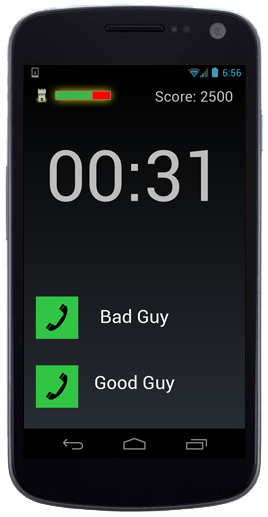
\includegraphics[width=0.14\textwidth]{kar}
\caption{The Starting page of mobile (Prototype}
\label{diagram}
\end{figure}
%-----------------------------------------------------------------


\bibliographystyle{unsrt}
\bibliography{refs}
\end{document}
